\section{Experiment}
\label{sec:experiment}

In this section, we describe experiments that empirically evaluate the proposed methods
described in Section~\ref{sec:method}, and compare with a few well known baseline approaches.

\cheng{There are a whole bunch of equations in Section 3. Define precisely what are the two methods that you present in your results tables. I.e. Write down sentences here, point to the relevant equation. Rework your method presentation such that you have one equation each for each one of multitask classification and multitask ranking.}

\subsection{Dataset}
We make use of two publicly available playlist dataset: the 30Music~\cite{30music2015} and AotM-2011~\cite{mcfee2012hypergraph} playlist dataset.
The Million Song Dataset~\cite{msd2011} serves as an underline dataset where all songs in playlists are intersected with,
it also provides a few features of songs which we will detail later.

{\bf Million Song Dataset} (MSD) is a collection of one million songs, information of each song such as the name, artist, year of release are available.
It also provides acoustic features computed from a sample section of audio file of each song. % more description

{\bf 30Music Dataset} is a collection of listening events and playlists retrieved from Last.fm\footnote{\url{https://www.last.fm}}.
We utilise the playlists data by first intersecting with the MSD, leveraging the Last.fm dataset~\cite{lastfmdataset}
which matched songs from Last.fm with those in MSD, then filtering out playlists with less than 5 songs,
which results in roughly 17K playlists over 45K songs from 8K users.

{\bf AotM-2011 Dataset} is a collection of playlists shared by users\footnote{\url{http://www.artofthemix.org}} ranging from 1998 to 2011,
songs in the dataset had been matched to those in the Million Song Dataset (MSD).
We filtered out playlists with less than 5 songs, which results in roughly 84K playlists over 114K songs from 14K users.

\cheng{Move dataset statistics into the appendix (Table 1-3). Unless you need it for something? It is not your dataset. I assume these statistics are in other papers already. Present statistics that describe something that justifies your method.}

Table~\ref{tab:stats_pldata} summarises the two playlist dataset used in this work.
%
\begin{table}[!h]
\centering
\caption{Music playlist dataset}
\label{tab:stats_pldata}
\resizebox{\linewidth}{!}{
\small
\begin{tabular}{lrcrcc}
\toprule
Dataset   & Songs & Playlists & Users & Songs/Playlist & Playlists/User \\
\midrule
30Music   & 45,468  & 17,457  & 8,070   & 16.3 & 2.2 \\
AotM-2011 & 114,428 & 84,710  & 14,182  & 10.1 & 6.0 \\
\bottomrule
\end{tabular}
}
\end{table}


\begin{figure}[h]
\centering
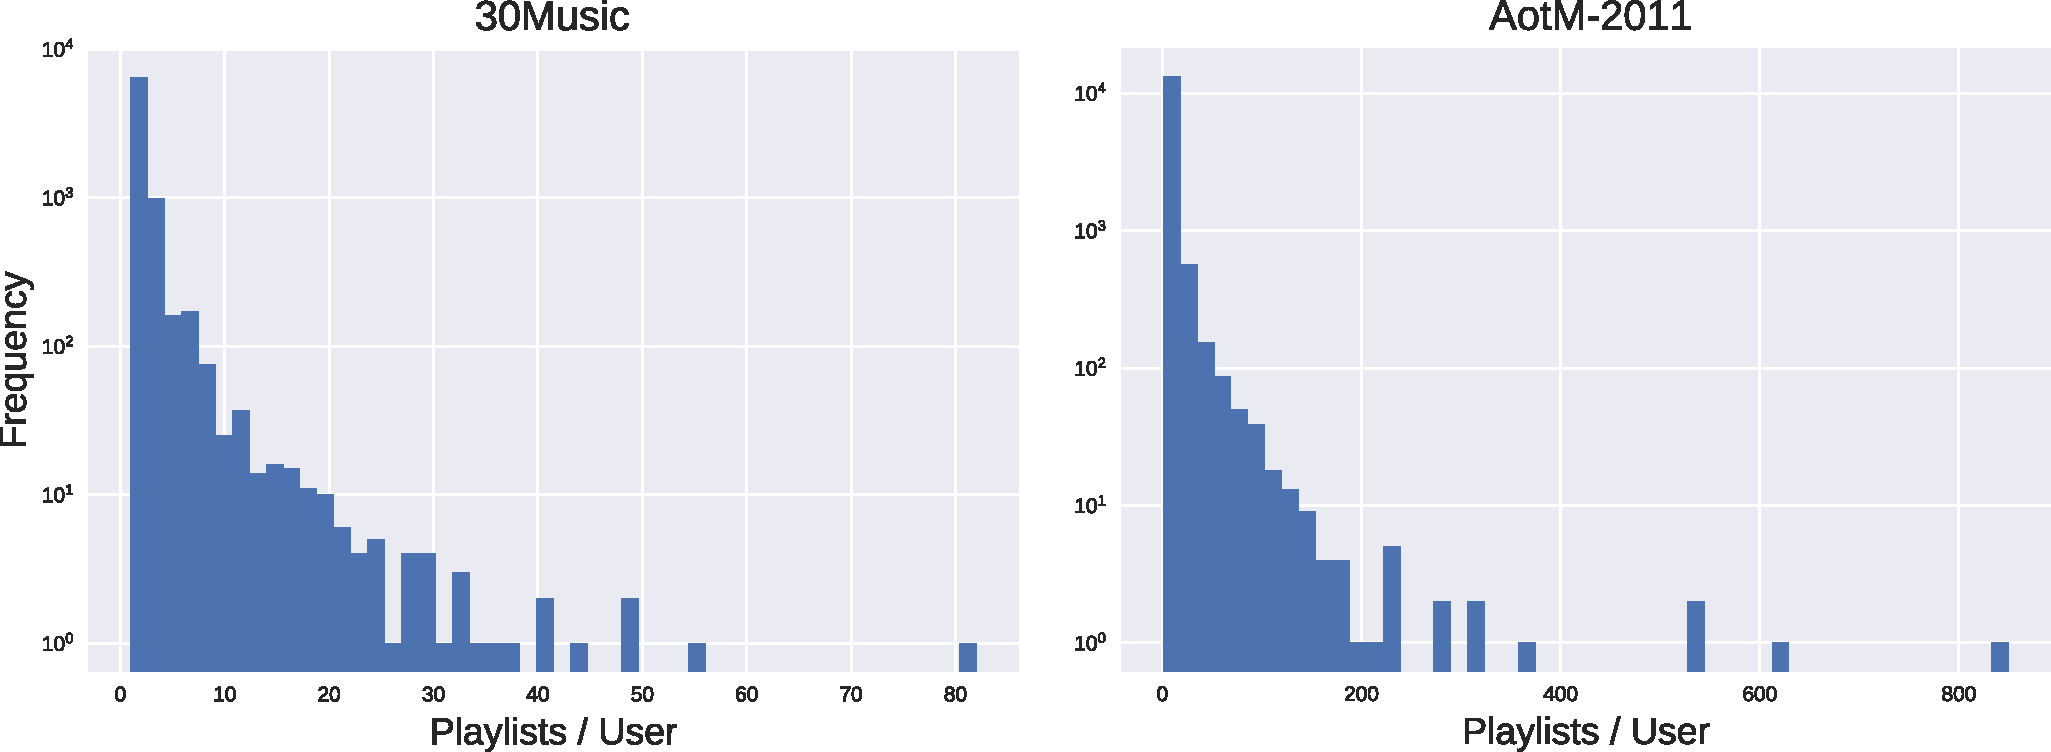
\includegraphics[width=\linewidth]{fig/hist_pluser.pdf}
\caption{Histogram of the number of playlists per user.}
\label{fig:hist_pluser}
\end{figure}

\begin{figure}[h]
\centering
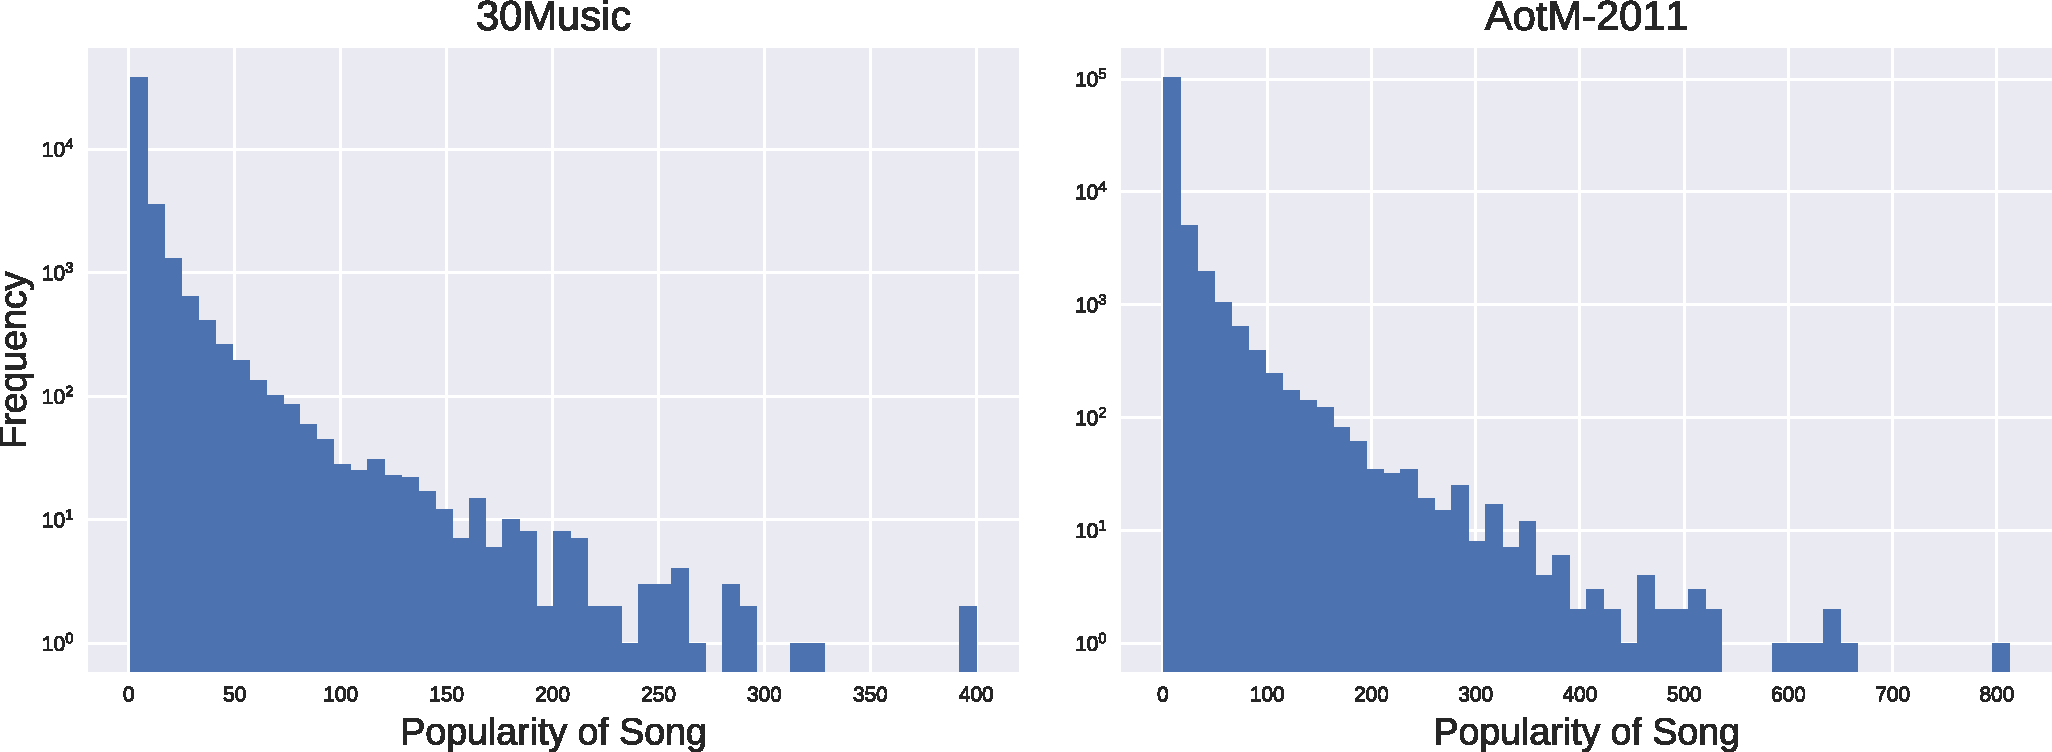
\includegraphics[width=\linewidth]{fig/hist_songpop.pdf}
\caption{Histogram of song popularity.}
\label{fig:hist_songpop}
\end{figure}

We can see from Figure~\ref{fig:hist_pluser} and \ref{fig:hist_songpop} that both the number
of playlists per user and song popularity (\ie the number of occurrences of a song in all playlists)
follow a long-tail distribution, which impose further challenge to the learning task as the amount
of data for learning is limited for users (or songs) at the tail.

\cheng{Describe what you did to prepare data that is not something that one can download. E.g. combining features.}

\subsection{Experimental setup}

{\bf Dataset split}.
To empirically evaluate the performance of our proposed recommendation approaches,
we hold 5K the latest released songs in 30Music dataset, which results in about 8K playlists with songs
in both training and test set.
We hold 10K the latest released songs in AotM-2011 dataset, which leads to about 19K playlists with songs
in both training and test set.
Playlists that all songs have been held are removed from both training and test set.

Table~\ref{tab:stats_nsr} summarises the statistics of this training/test split.

\begin{table}[!h]
\centering
\caption{Dataset of new song recommendation}
\label{tab:stats_nsr}
\begin{tabular}{lrrcrr}
\toprule
\multirow{2}{*}{Dataset}  & \multicolumn{2}{c}{Songs} && \multicolumn{2}{c}{Playlists} \\ \cmidrule{2-3} \cmidrule{5-6}
                          & Train & Test && Train & Test \\
\midrule
30Music   & 40,468  & 5,000  && 17,342  & 8,215 \\
AotM-2011 & 104,428 & 10,000 && 84,646  & 19,504 \\
\bottomrule
\end{tabular}
\end{table}




We describe how playlist data are split in training and test set,
features of songs used to learn the multitask objective, as well as
baseline approaches and evaluation metrics.

{\bf Dataset split}.
To empirically evaluate the performance of our proposed recommendation approaches for existing users,
we hold playlists from about 20\% users in both datasets for test,
all other playlists are used for training.
To make sure each song in test set also appeared in training set,
and all users in test set also have a few playlists in training set.
The test set are sampled from users that have at least one playlist where each song has also been
included in four other playlists among the whole dataset,
which results in a test set with about 2.1K playlists from 1.6K users in 30Music dataset,
and a test set with about 9.2K playlists from 2.7K users in AotM-2011 dataset.
The statistics of this training/test split are shown in Table~\ref{tab:stats_warm}.

\begin{table}[!h]
\centering
\caption{Dataset of recommendation for existing users}
\label{tab:stats_warm}
\begin{tabular}{lrrcrr}
\toprule
\multirow{2}{*}{Dataset}  & \multicolumn{2}{c}{Playlists} && \multicolumn{2}{c}{Users} \\ \cmidrule{2-3} \cmidrule{5-6}
                          & Train & Test && Train & Test \\
\midrule
30Music   & 15,262 & 2,195 &&  8,070 & 1,644 \\
AotM-2011 & 75,477 & 9,233 && 14,182 & 2,722 \\
\bottomrule
\end{tabular}
\end{table}

To evaluate the performance of music recommendation approaches for new users,
we sampled 30\% of all users and hold all their playlists as test set in both datasets.
Similarly, to make sure songs in test set also exist in training set,
a user is not sampled when holding all of her playlists breaks this requirement.
This results in a test set with about 3.4K playlists from 2.4K users in 30Music dataset,
and a test set with about 8.2K playlists from 4.2K users in AotM-2011 dataset.
The statistics of this training/test split can be found in Table~\ref{tab:stats_cold}.

\begin{table}[!h]
\centering
\caption{Dataset of recommendation for new users}
\label{tab:stats_cold}
\begin{tabular}{lrrcrr}
\toprule
\multirow{2}{*}{Dataset}  & \multicolumn{2}{c}{Playlists} && \multicolumn{2}{c}{Users} \\ \cmidrule{2-3} \cmidrule{5-6}
                          & Train & Test && Train & Test \\
\midrule
30Music   & 14,067 & 3,390 && 5,649 & 2,421 \\
AotM-2011 & 76,450 & 8,260 && 9,928 & 4,254 \\
\bottomrule
\end{tabular}
\end{table}


{\bf Features} of each song used in experiment including metadata, audio data, genre, artist information and song popularity.
Song metadata (\eg duration, year of release) and audio features (\eg loudness, mode, tempo) are provided by MSD.

We also make use of genre data from the Top-MAGD genre dataset~\cite{schindler2012facilitating}
and tagtraum genre annotations for MSD~\cite{schreiber2015improving} via one-hot encoding.
If the genre data of a song is not available, we apply the mean imputation using genre counts of other songs in training set.
To encode artist information as features,
we trained a word2vec\footnote{https://github.com/dav/word2vec} model using sequences of artist names in playlists.

Finally, we add a constant feature (with value $1$) for each song to account for bias, and song popularity is included as well.


{\bf Baselines}.
We compare the performance of our proposed approaches with a few baseline approaches
that were known to work well on the task of recommending music to form playlists.

Firstly, the {\it Popularity Rank} method, which scores each song using only its popularity in training set.
%
Another approach that based on song popularity and artist is the {\it Same Artists - Greatest Hits} (SAGH)~\cite{mcfee2012million} method,
which scores each song by its popularity if the artist of the song has appeared in the given user's playlist in training set,
otherwise the song is scored zero.
%
The {\it Collocated Artists - Greatest Hits} (CAGH)~\cite{bonnin2013evaluating} method is a variant of SAGH
that also scores each song using its popularity, but weighted by the frequency of the collocation between artist of the song
and those artists that appeared in the given user's playlist in training set.

The {\it Popularity Rank} approach is readily available to be a baseline for the setting of recommending music for new users.
%
We slightly modified the SAGH and CAGH approaches so that they can also work in this setting,
in particular, we replace artists that appeared in user's training playlists in the previous setting with the 10 most popular artists
(we use the number of occurrences of all songs from a artist in training playlists as a proxy of her popularity),
and refer these two approaches as Top10 SAGH and Top10 CAGH, respectively.

\cheng{Independent logistic regression. What is single task?}

\cheng{Why don't we compare to matrix factorization?}

{\bf Evaluation}.
We evaluate performance of all approaches using three metrics that are commonly employed in music recommendation for playlist tasks:
R-Precision~\cite{manning2008introIR}, Hit-Rate@K~\cite{hariri2012context} and Area under the ROC curve (AUC)~\cite{manning2008introIR}.

R-Precision (RPREC) is the number of correctly recommended songs in the top-$n$ recommendation over $n$,
where $n$ is the number of songs in the ground truth playlist.
It is one of several metrics used to evaluate performance on playlist continuation tasks
in the ACM RecSys Challenge 2018\footnote{https://recsys-challenge.spotify.com/rules}.
%
Hit-Rate@K (or Hit Ratio) is the number of correctly recommended songs among top-$K$ recommendation over $n$,
where $K$ is the number of recommendations, and $n$ is the number of songs in the ground truth playlist as before.
It has been employed to evaluate several playlist generation and next song recommendation
methods~\cite{hariri2012context,bonnin2013evaluating,bonnin2015automated,jannach2015beyond}.
%
The area under the ROC curve (AUC) is widely used in measuring performance of classifiers,
it has also been used for evaluating performance of playlist generation method when the task
is cast as a sequential classification problem~\cite{ben2017groove}.

\cheng{Describe why CAGH does well on one metric and not the other.}

\subsection{Results and discussion}


\begin{table}[t]
\centering
\caption{Performance of new song recommendation}
\label{tab:perf0}
\resizebox{\columnwidth}{!}{
\begin{tabular}{l*{4}{c}*{4}{c}}
\toprule
\multirow{2}{*}{Method}      & \multicolumn{2}{c}{30Music} && \multicolumn{2}{c}{AotM-2011} \\ \cmidrule{2-3} \cmidrule{5-6}
                             & HitRate@100 \% & AUC \% && HitRate@100 \% & AUC \% \\
\midrule
SAGH &                   \hspace{0.45em}$4.8$ & $51.6$ && \hspace{0.2em} $7.8$ & $53.6$ \\
CAGH &                                 $10.9$ & $69.2$ &&               $11.9$ & $77.5$ \\
Popularity Ranking &                   $12.2$ & $70.9$ && \hspace{0.2em} $8.7$ & $76.5$ \\
Logistic Regression &                  $35.4$ & $82.5$ &&               $23.1$ & $81.0$ \\
Multitask Classification & ${\bf 36.2}$ & ${\bf 86.6}$ &&         ${\bf 24.4}$ & ${\bf 84.3}$ \\
\bottomrule
\end{tabular}

}
\end{table}

\begin{figure}[t]
\centering
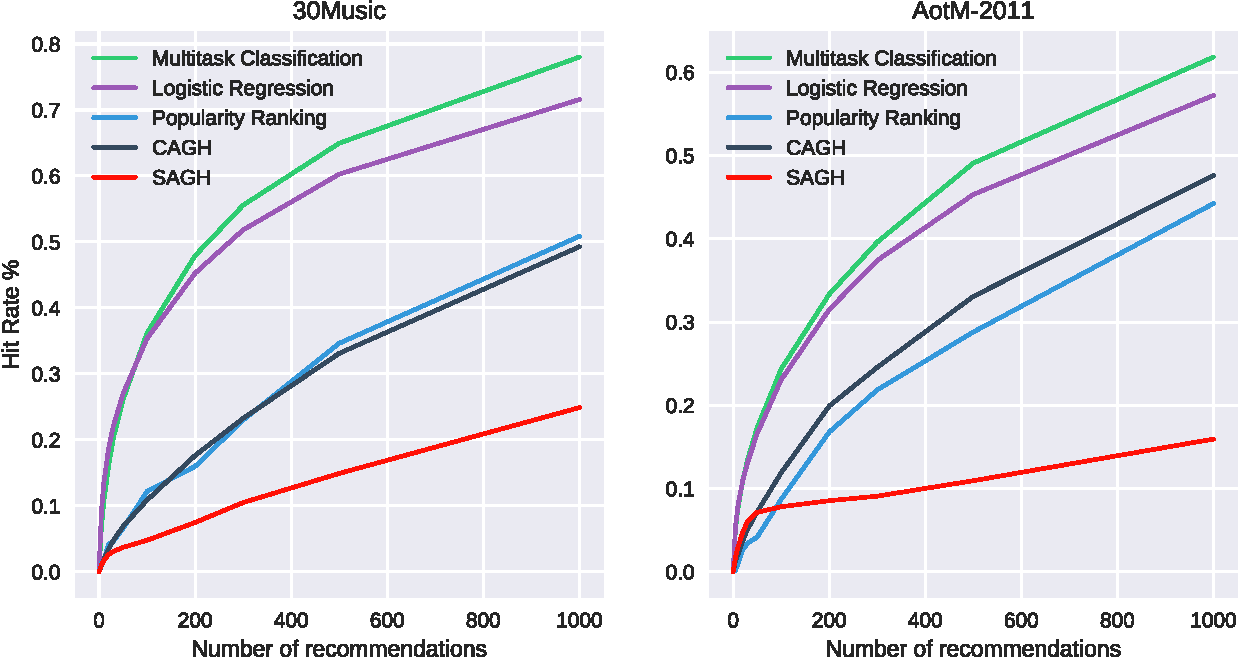
\includegraphics[width=\linewidth]{fig/hitrate0.pdf}
\caption{Hit rates of new song recommendation.}
\label{fig:hr0}
\end{figure}





We first compare the performance of music recommendation to form playlist for existing users.

Table~\ref{tab:perf1} and Figure~\ref{fig:hr1} show that simply ranking songs by popularity (\ie {\it Popularity Rank})
can achieve decent performance,
it outperforms SAGH in terms of both AUC and Hit-Rate (when the number of recommendations are greater than 350) on 30Music,
and also performs better in term of AUC on AotM-2011 dataset.
This is in line with discoveries in~\cite{bonnin2013evaluating,jannach2015beyond,bonnin2015automated} that show ranking based on
popularity is a strong baseline.
Further, we note that methods which make use of both song popularity and artist information,
outperform {\it Popularity Rank} on both datasets (except SAGH on 30Music), which shows artist information is helpful for music recommendation.
This is consistent with the results reported in~\cite{bonnin2013evaluating,bonnin2015automated}.
Lastly, our proposed methods, both the ranking and classification approaches, consistently outperforms all baselines
on both datasets and in terms of all metrics, which shows the proposed multitask learning objective works effectively
in the setting of music recommendation for existing users.

\begin{table}[t]
\centering
\caption{Performance of recommendation for existing users}
\label{tab:perf1}
\resizebox{\columnwidth}{!}{
\begin{tabular}{l*{4}{c}*{4}{c}}
\toprule
\multirow{2}{*}{Method}      & \multicolumn{2}{c}{30Music} && \multicolumn{2}{c}{AotM-2011} \\ \cmidrule{2-3} \cmidrule{5-6}
                             & HitRate@100 \% & AUC \% && HitRate@100 \% & AUC \% \\
\midrule
SAGH &                   \hspace{0.45em}$4.8$ & $51.6$ && \hspace{0.2em} $7.8$ & $53.6$ \\
CAGH &                                 $10.9$ & $69.2$ &&               $11.9$ & $77.5$ \\
Popularity Ranking &                   $12.2$ & $70.9$ && \hspace{0.2em} $8.7$ & $76.5$ \\
Logistic Regression &                  $35.4$ & $82.5$ &&               $23.1$ & $81.0$ \\
Multitask Classification & ${\bf 36.2}$ & ${\bf 86.6}$ &&         ${\bf 24.4}$ & ${\bf 84.3}$ \\
\bottomrule
\end{tabular}

}
\end{table}


\begin{figure}[t]
\centering
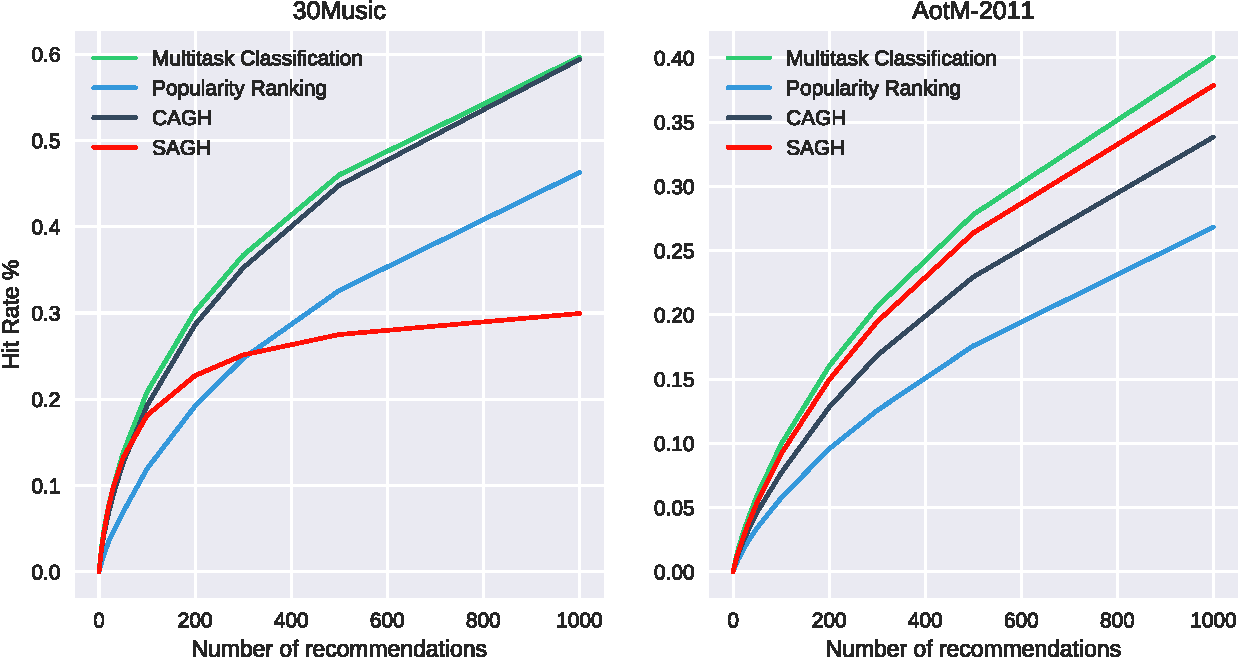
\includegraphics[width=\linewidth]{fig/hitrate1.pdf}
\caption{Hit rates of recommendation for existing users.}
\label{fig:hr1}
\end{figure}

\cheng{Explain why HR@K is different for the two datasets, at least for the baselines. Might need a new small experiment.}

Performance in the setting of recommending music to form playlists for new users,
however, is quite different from recommendation for existing users.

We can see from Table~\ref{tab:perf2} and Figure~\ref{fig:hr2} that {\it Popularity Rank} is one of the best performing methods,
outperforming two baselines that make use of both popularity and artist information (\ie Top10 SAGH and Top10 CAGH).
Our proposed methods perform comparably to {\it Popularity Rank}, which might suggest that they degenerate to simply use popularity to rank songs.
Further, it is interesting to observe that, although both Top10 SAGH and Top10 CAGH make use of song popularity and artist information,
the later performs significantly better than the former in terms of AUC and Hit-Rate.
This shows the way to make use of artist information matters,
and collocation of artists could be more helpful than simply filtering out songs by familiar/popular artists
with regards to music recommendation.

Another observation is that performance (in terms of Hit-Rate) of all methods improve as the number of recommendations increase,
and the rate of improvement decrease as more songs are recommended.
In particular, the improvement of (Top10) SAGH tends to saturate much earlier than other methods
(except recommendations on AotM-2011 dataset for existing users),
which might imply that, as more songs are recommended, the artists in users' listening history
(or most popular artists) become less informative,
and other factors such as song popularity regains its dominance in music prediction.

\begin{table}[t]
\centering
\caption{Performance of recommendation for new users}
\label{tab:perf2}
\resizebox{\columnwidth}{!}{
%\begin{table}[!h]
%\centering
%\caption{Performance of recommendation for new users}
%\label{tab:perf_plgen2}
%\resizebox{\columnwidth}{!}{
\begin{tabular}{l*{4}{c}*{4}{c}}
\toprule
\multirow{2}{*}{Method}  & \multicolumn{2}{c}{30Music} && \multicolumn{2}{c}{AotM-2011} \\ \cmidrule{2-3} \cmidrule{5-6}
                         & RPREC \textperthousand & AUC \% && RPREC \textperthousand & AUC \% \\
\midrule
Popularity Rank &           $21.4$ & $88.3$ &&                       $13.5$ & $91.8$ \\
Top10 SAGH &                $19.6$ & $54.5$ &&                       $11.5$ & $53.7$ \\
Top10 CAGH &                $19.5$ & $87.3$ &&                       $11.5$ & $89.4$ \\
Multitask Classification &  $21.0$ & $88.8$ &&                       $13.5$ & $91.6$ \\
Multitask Ranking &            N/A &    N/A &&                          N/A &    N/A \\
\bottomrule
\end{tabular}
%}
%\end{table}

}
\end{table}

\cheng{Explain why popularity works well for RPREC for new users as compared to existing users.}

\begin{figure}[t]
\centering
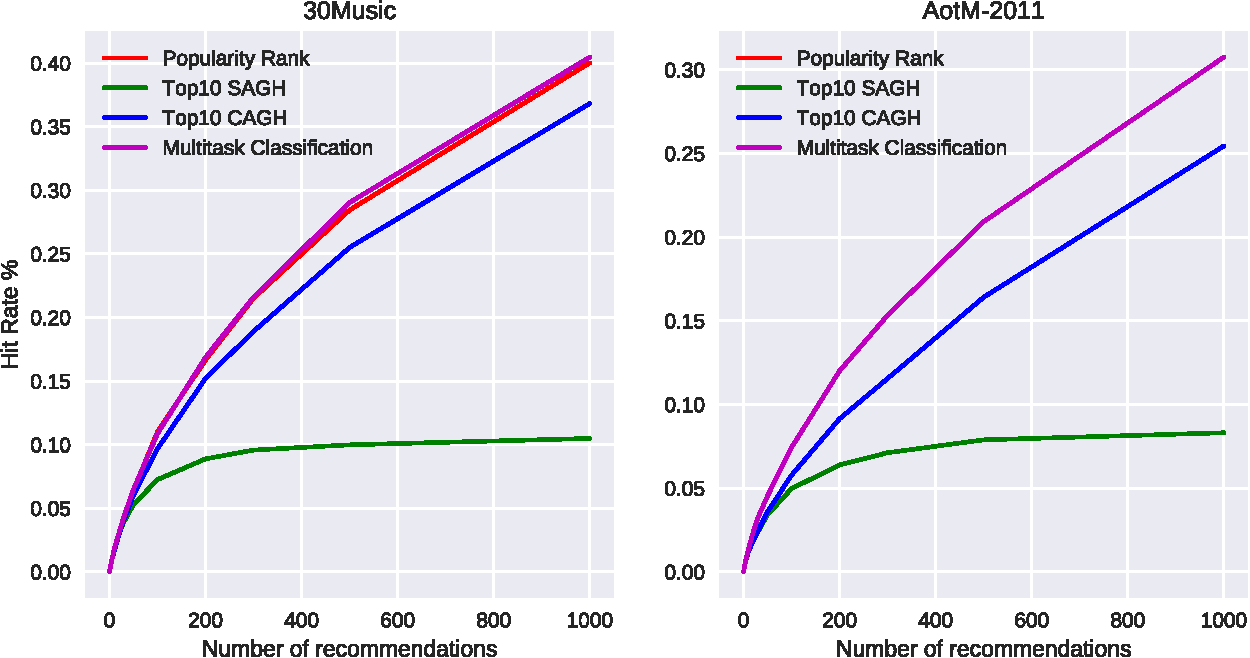
\includegraphics[width=\linewidth]{fig/hitrate2.pdf}
\caption{Hit rates of recommendation for new users.}
\label{fig:hr2}
\end{figure}

\cheng{Add a discussion about the ablation experiment. Discuss user specific vs user agnostic predictions.}
